\chapter{Introduzione a gem5 e RISC-V}

\section{Il Simulatore gem5}
Durante il corso utilizzeremo \textbf{gem5}, un simulatore architetturale e micro-architetturale open source. Lo scopo principale di questo strumento è permetterci di valutare come specifiche scelte micro-architetturali impattino le prestazioni complessive di un sistema.

\begin{definition}[Simulatore gem5]
gem5 è un simulatore di livello sistema e micro-architetturale che supporta varie architetture ISA (Instruction Set Architecture), tra cui ARM, x86 e RISC-V. Permette di simulare un intero sistema offrendo un controllo a grana fine su tutti i suoi componenti (sistema di cache, branch prediction, unità funzionali della CPU).
\end{definition}

Nella nostra configurazione, utilizzeremo gem5 per eseguire programmi scritti in \textbf{assembly RISC-V}. Non faremo girare un sistema operativo completo (configurazione \textit{bare metal}); il processore eseguirà direttamente il nostro codice. 

Il simulatore è estremamente flessibile: è scritto principalmente in C++ (per i moduli eseguibili) ed è configurabile tramite script Python. Modificando i parametri negli script Python, potremo cambiare le caratteristiche delle unità funzionali (es. le latenze) e osservare come variano i tempi di esecuzione.

\subsection{La Pipeline a 5 Stadi}
L'architettura CPU che utilizzeremo in gem5 è stata sviluppata specificamente per questo corso e rispecchia fedelmente la classica \textbf{pipeline a 5 stadi} descritta da Hennessy e Patterson:
\begin{enumerate}
    \item \textbf{Fetch} (F): Prelevamento dell'istruzione dalla memoria.
    \item \textbf{Decode} (D): Decodifica dell'istruzione e lettura dei registri.
    \item \textbf{Execute} (E): Esecuzione dell'operazione nell'ALU.
    \item \textbf{Memory} (M): Accesso alla memoria dati (se necessario).
    \item \textbf{Writeback} (W): Scrittura del risultato nel file dei registri.
\end{enumerate}

% FIGURA DA INSERIRE QUI
% Fonte: Slide "Gem5 - 3 RISC-V 5-stage pipeline"
% Descrizione: Diagramma temporale della pipeline a 5 stadi con l'avanzamento dei cicli di clock.
\begin{figure}[H]
    \centering
    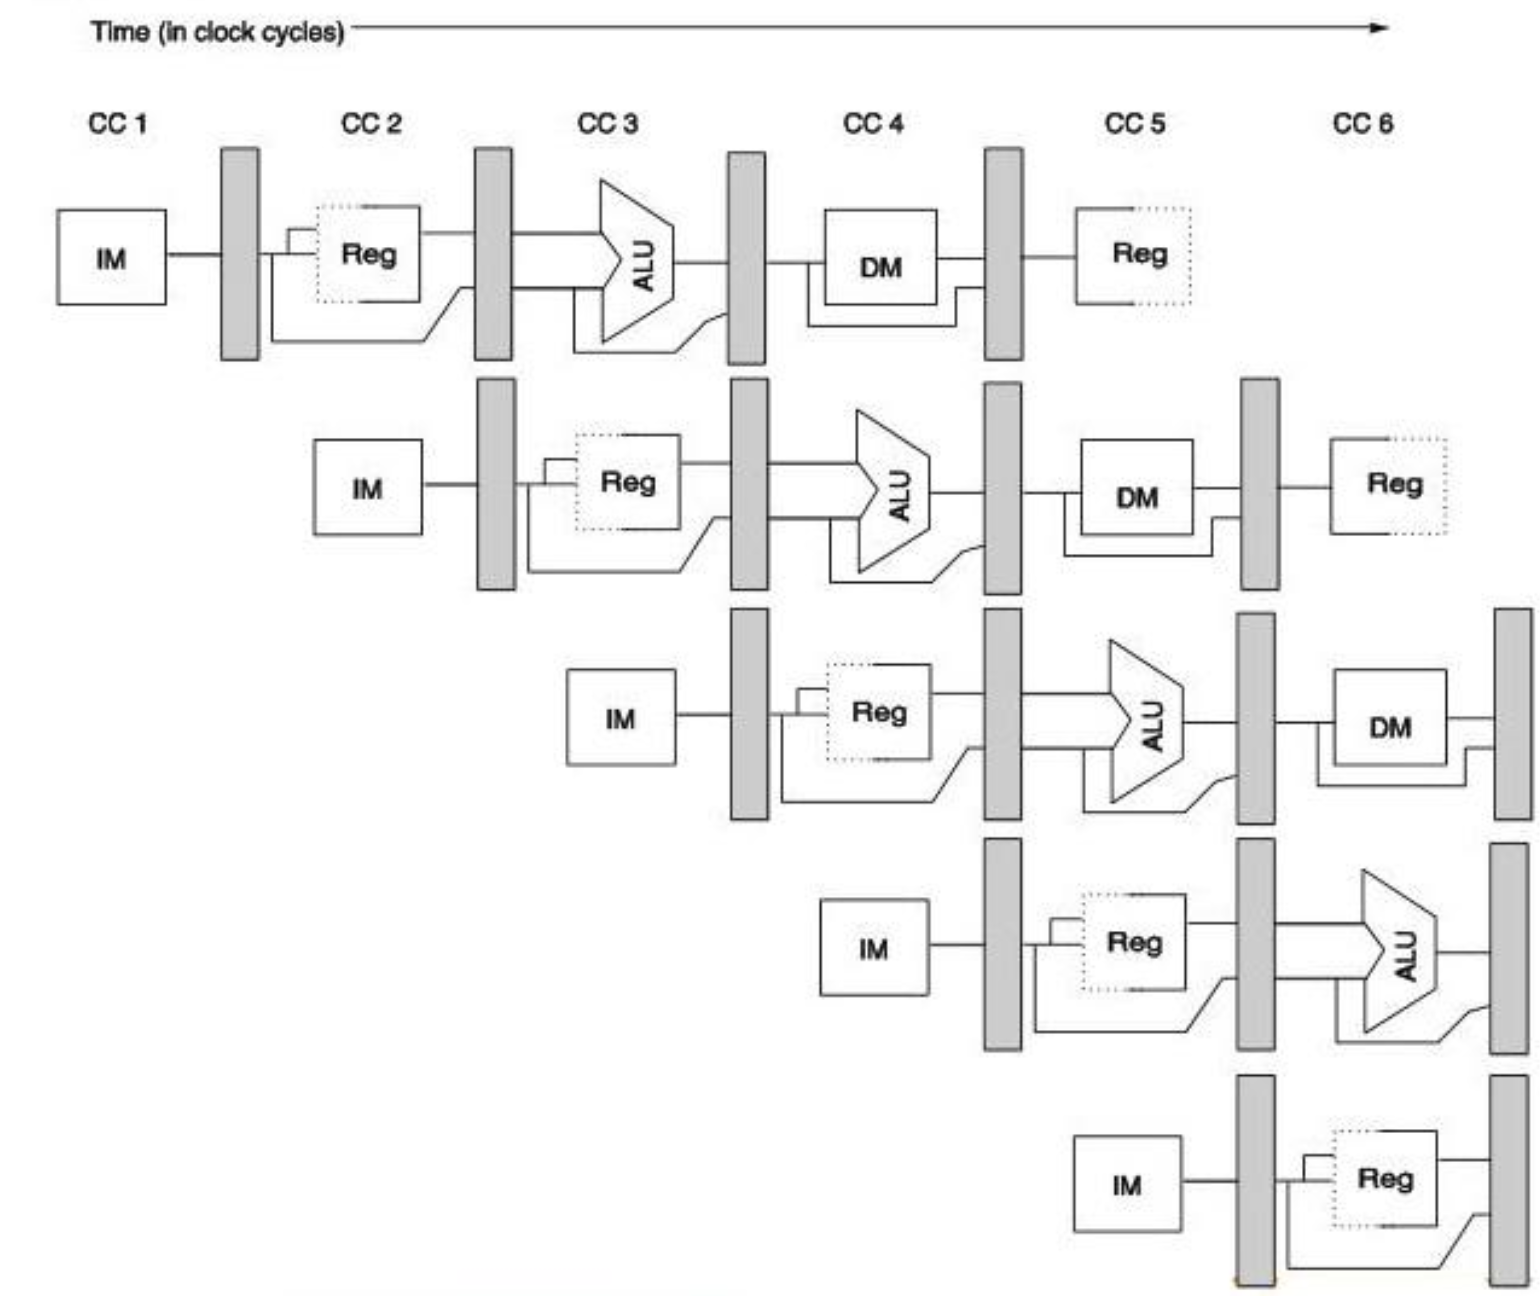
\includegraphics[width=0.6\textwidth]{capitoli/04_gem5/images/riscv_pipeline.png}
    \caption{Rappresentazione dei 5 stadi della pipeline RISC-V.}
    \label{fig:riscv_pipeline}
\end{figure}

\section{Struttura dei Programmi in Assembly}
L'architettura di riferimento implementa il modello \textbf{Load/Store} e si basa su un'architettura \textbf{Harvard}, in cui la memoria dati e la memoria istruzioni sono separate e collegate esternamente al processore. Questo è fondamentale per le prestazioni, in quanto permette alla CPU di accedere simultaneamente a entrambe le memorie nello stesso ciclo di clock.

Coerentemente con questa divisione fisica, anche a livello logico i nostri programmi in assembly (tipicamente salvati con estensione \texttt{.s}) saranno divisi in due sezioni principali tramite specifiche direttive per il compilatore:

\begin{itemize}
    \item \texttt{.data} (o \texttt{.section .data}): È la sezione dedicata ai dati. Qui vengono allocate le variabili, i vettori e le costanti che risiederanno nella memoria dati. 
    \item \texttt{.text} (o \texttt{.code} / \texttt{.section .text}): È la sezione che contiene il codice del programma vero e proprio (routine, sottoroutine, funzioni) che risiederà nella memoria istruzioni.
\end{itemize}

\begin{remark}[L'importanza dei commenti e dell'indentazione]
Le istruzioni assembly sono talmente elementari che il loro scopo di alto livello (es. moltiplicare per 8 tramite uno shift) si perde facilmente. Il professore sottolinea che \textbf{commentare il codice} (es. spiegare cosa si sta facendo a livello logico, mappare i registri alle variabili) è obbligatorio, specialmente in sede d'esame. Inoltre, le istruzioni vanno sempre indentate (con un tab o 4 spazi) lasciando le etichette (labels) a margine sinistro per garantirne la leggibilità.
\end{remark}

\section{Confronto Prestazionale: RISC vs CISC}
Per capire l'impatto del set di istruzioni sull'architettura, analizziamo un semplice frammento di codice che esegue l'operazione \( C = A + B \) in memoria, confrontando un approccio RISC (RISC-V) e un approccio CISC (Intel 8086).

\begin{example}[Somma di due variabili in memoria]
In RISC-V, non è possibile sommare direttamente un elemento di memoria con un registro. Bisogna prima caricare i dati nei registri (Load), eseguire la somma, e salvare il risultato (Store).

\begin{figure}[H]
    \centering
    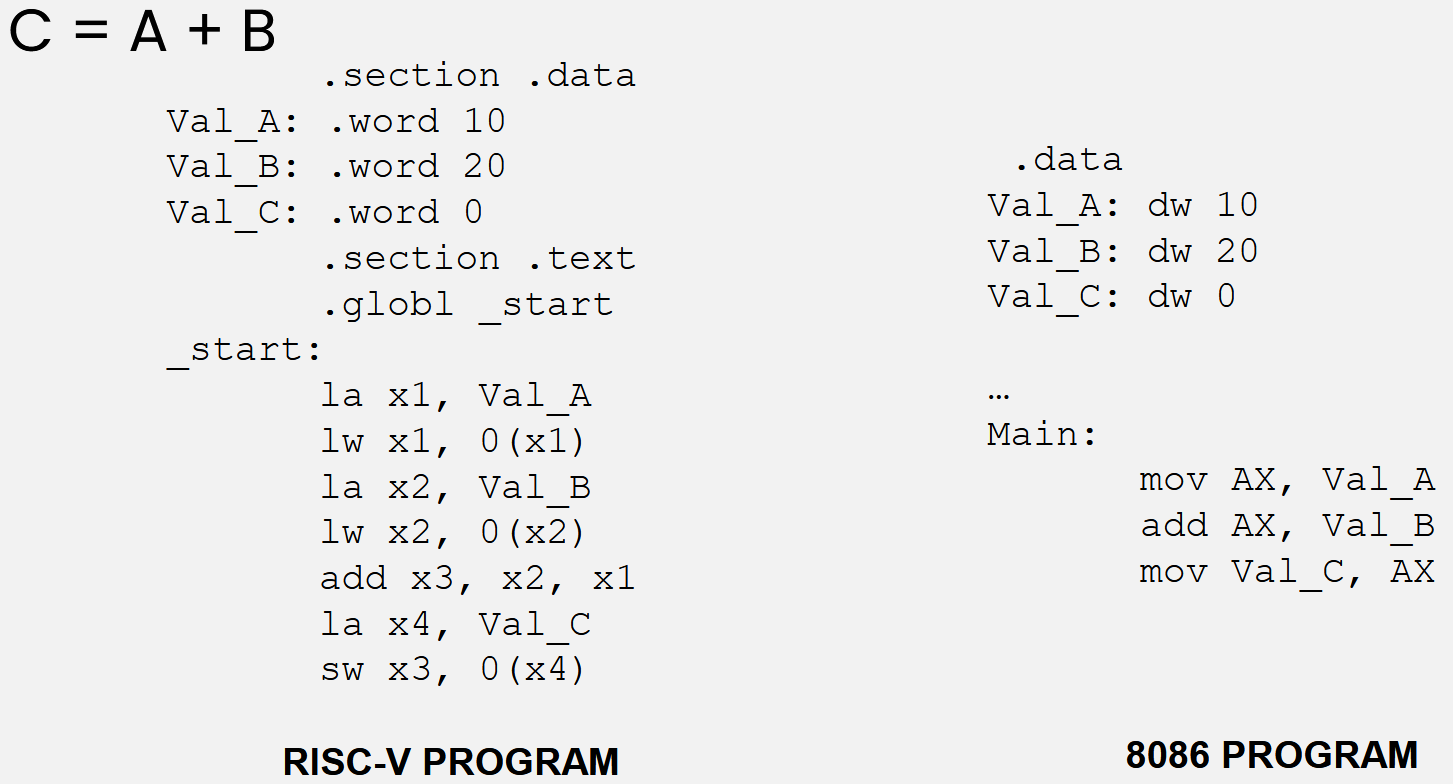
\includegraphics[width=0.8\textwidth]{capitoli/04_gem5/images/riscv_vs_8086.png}
    \caption{Confronto tra RISC-V (Load/Store) e 8086 (CISC) per l'operazione \( C = A + B \).}
    \label{fig:riscv_vs_8086}
\end{figure}

Nel 8086 (CISC), un'istruzione può includere sia l'operazione aritmetica sia l'accesso alla memoria:

\end{example}

\begin{table}[H]
    \centering
    \begin{tabular}{lcc}
        \toprule
        \textbf{Metrica} & \textbf{RISC-V (Load/Store)} & \textbf{8086 (CISC)} \\
        \midrule
        Numero di istruzioni & 7 (10 con espansione pseudo-istr.) & 3 \\
        Dimensione codice & 40 byte & 8 byte \\
        Tempo di esecuzione & \textbf{15 Cicli di Clock} & \textbf{33 Cicli di Clock} \\
        \bottomrule
    \end{tabular}
    \caption{Confronto tra approccio RISC e CISC per l'operazione $C = A + B$.}
    \label{tab:risc_vs_cisc}
\end{table}

\begin{remark}[Analisi del confronto]
Anche se il programma CISC è molto più compatto (meno istruzioni e meno byte), l'architettura RISC impiega meno cicli di clock per terminare l'elaborazione. Nel CISC, infatti, la complessa gestione interna necessaria per accedere alla memoria e fare calcoli nella stessa istruzione rallenta notevolmente l'esecuzione complessiva. Oggi, la maggior parte dei processori CISC traduce internamente le istruzioni complesse in micro-istruzioni di tipo RISC.
\end{remark}

\section{Ambiente di Sviluppo e Simulazione}
Per sviluppare e testare il codice, il ciclo di lavoro prevede tre fasi:
\begin{enumerate}
    \item \textbf{Compilazione:} Si utilizza la toolchain \texttt{gcc} per RISC-V (comando \texttt{riscv\_compile}).
    \item \textbf{Simulazione:} Si esegue il simulatore passandogli lo script Python di configurazione, l'eseguibile e il nome del file di log di output (comando \texttt{gem5\_run gem5\_config.py program program.log}).
    \item \textbf{Visualizzazione:} Tramite \textbf{ASE Studio} (o \texttt{gem5\_pipeline\_visualizer}), si apre il log generato.
\end{enumerate}

ASE Studio è un IDE interattivo che integra tutto l'esperimento: permette di editare il progetto, compilare, simulare e ispezionare visivamente la pipeline.

% FIGURA DA INSERIRE QUI
% Fonte: Slide "ASE Studio V1.0.0 - 5" (o una qualsiasi schermata generale di ASE Studio)
% Descrizione: Interfaccia utente di ASE Studio con editor a sinistra e diagramma pipeline in basso.
\begin{figure}[H]
    \centering
    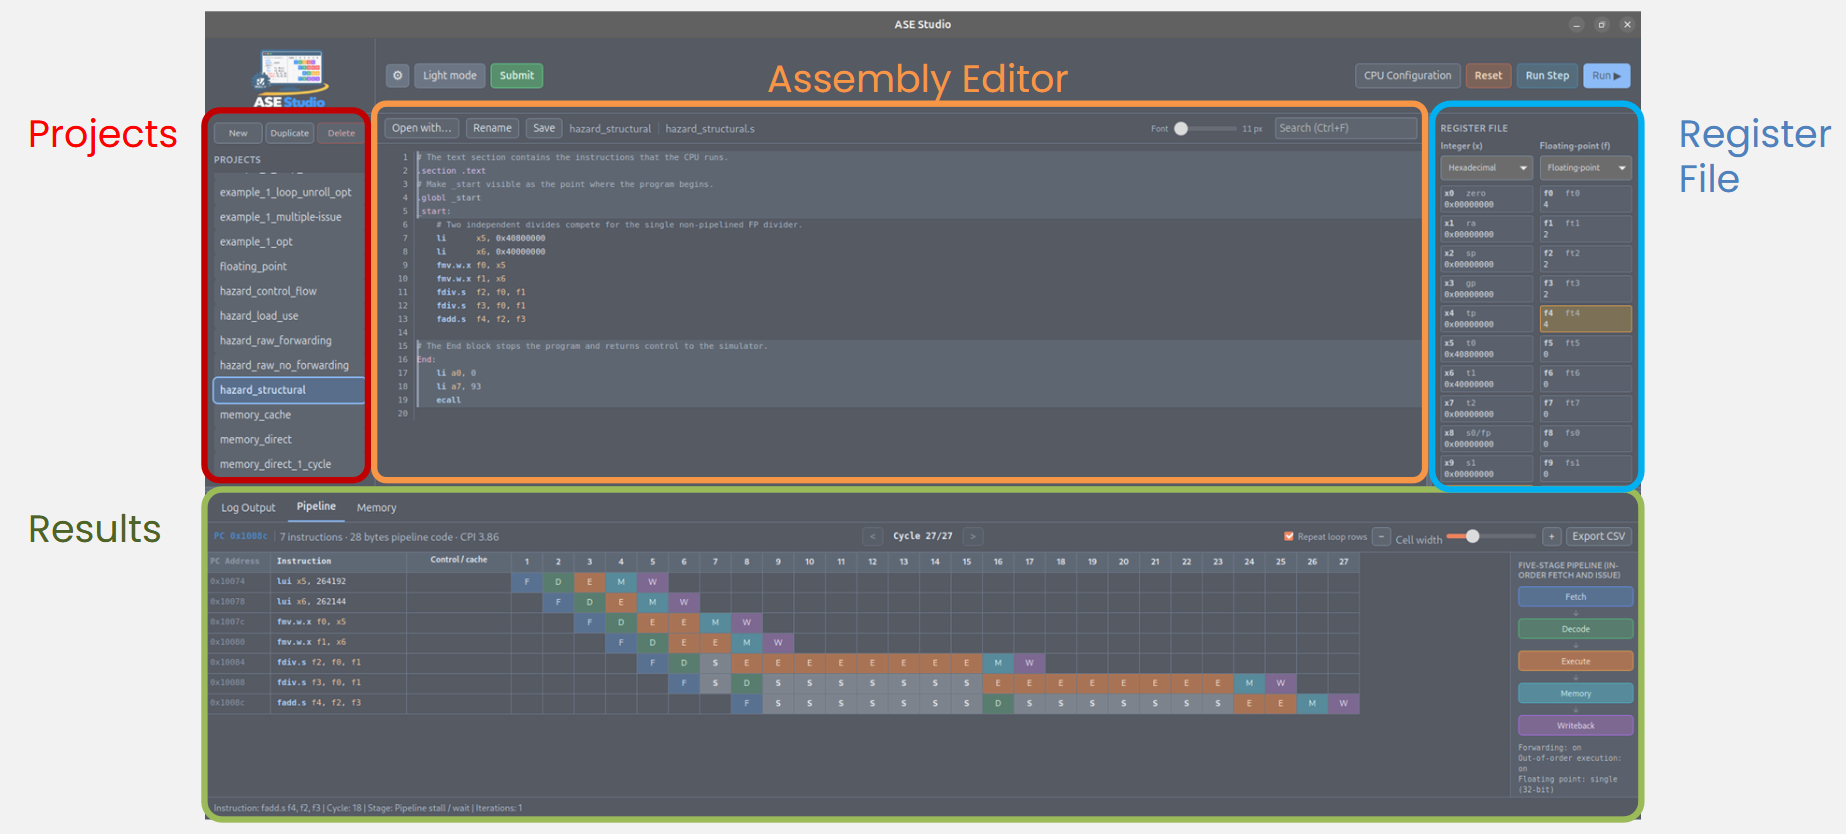
\includegraphics[width=0.9\textwidth]{capitoli/04_gem5/images/ase_studio_interface.png}
    \caption{Interfaccia di ASE Studio: Editor del codice, pipeline a griglia e stato dei registri.}
    \label{fig:ase_studio}
\end{figure}

Nella vista della pipeline, ogni riga rappresenta un'istruzione e ogni colonna un ciclo di clock, evidenziando come l'istruzione attraversa gli stadi (F, D, E, M, W) ed eventuali stalli (S). Sulla destra è visibile lo stato del \textit{Register File} (registri interi \texttt{x} e floating-point \texttt{f}).

Poiché il visualizzatore legge un log di una simulazione \textit{già terminata}, \textbf{non è possibile modificare i dati in memoria o nei registri al volo} durante l'osservazione.

\section{Stesura di un Programma: Pratiche Fondamentali}
Quando si scrive un programma da valutare nel simulatore gem5, bisogna tenere a mente che stiamo misurando le prestazioni architetturali (latenze della pipeline, data hazard, etc.). 

\subsection{Il problema del Cache Miss iniziale}
Nella realtà, il primo accesso a un dato in memoria richiede un trasferimento dalla memoria principale (RAM) alla memoria Cache, operazione che impiega decine o centinaia di cicli di clock. Se misurassimo il programma fin dalla prima istruzione, le nostre statistiche prestazionali sarebbero dominate e "sporcate" da questi ritardi iniziali di accesso in memoria, impedendoci di valutare l'efficienza della nostra struttura della pipeline.

Per ovviare a questo problema, si utilizza una tecnica di \textbf{pre-riscaldamento (warming) della cache}. Le linee di cache nel simulatore sono state configurate per essere molto grandi. Basterà quindi fare una \textit{lettura a vuoto} del primo elemento di un vettore affinché l'intero blocco dati venga caricato in cache.

\subsection{L'etichetta \texttt{\_start} e la struttura del codice}
Essendo in configurazione \textit{bare metal} senza sistema operativo, il punto di ingresso \textbf{deve} chiamarsi \texttt{\_start} (non \texttt{main} né \texttt{START}). 
Sotto questa etichetta scriveremo il "prologo" per precaricare i dati, seguito da dei \texttt{nop} per attendere che i dati arrivino effettivamente in cache (circa 4-6 cicli di clock). Solo a quel punto inseriremo l'etichetta del \texttt{main} vero e proprio, da dove inizieremo a misurare le prestazioni.

\begin{example}[Somma di due Vettori con Cache Warming]
Di seguito un esempio per sommare due vettori (\texttt{V1} e \texttt{V2}) e salvare il risultato in un terzo vettore (\texttt{result}). 

\begin{verbatim}
.section .data
V1: .word 1, 2, 3, 4, 5, 6, 7, 8, 9, 10
V2: .word 1, 2, 3, 4, 5, 6, 7, 8, 9, 10
result: .space 40   # Alloca 40 byte (10 word) senza inizializzarli

.section .text
.globl _start

_start:
# --- PROLOGO: RISCALDAMENTO CACHE ---
la x1, V1
la x2, V2
la x3, result
lw x0, 0(x1)  # Legge il primo el. di V1 (carica in cache)
lw x0, 0(x2)  # Legge il primo el. di V2 (carica in cache)
# (Il caricamento usa registri temporanei o x0, il dato non ci serve ora)
nop
nop
nop

main:
# --- INIZIO PROGRAMMA REALE ---
la x1, V1
la x2, V2
la x3, result
addi x4, x0, 10  # Contatore ciclo (10 iterazioni)

cycle:
lw x5, 0(x1)     # Legge da V1
lw x6, 0(x2)     # Legge da V2
add x7, x5, x6   # Somma
sw x7, 0(x3)     # Salva in result

# Aggiornamento indici (indirizzi byte-addressable -> +4)
addi x1, x1, 4
addi x2, x2, 4
addi x3, x3, 4
addi x4, x4, -1  # Decrementa contatore
bnez x4, cycle   # Salta a cycle se x4 != 0

END_of_PROGRAM:
# --- EPILOGO: SYSTEM CALL EXIT ---
li a0, 0         # Valore di ritorno 0
li a7, 93        # Codice syscall per exit()
ecall
\end{verbatim}
\end{example}

\begin{remark}[Osservazioni sul codice]
Si noti che l'aggiornamento degli indici del vettore avviene sommando 4 (e non 1 come avverrebbe in linguaggio C). Questo perché la memoria è indirizzabile al byte (\textit{byte-addressable}) e ogni numero intero (\texttt{.word}) in RISC-V occupa 32 bit, ovvero 4 byte. 
Per concludere correttamente la simulazione gem5 senza far crashare il sistema, il programma deve terminare con una System Call di \texttt{exit} (passando 93 al registro \texttt{a7} ed eseguendo \texttt{ecall}).
\end{remark}